\documentclass[main.tex]{subfiles}
\begin{document}
\subsection{Day 11: 9/16/22}
\subsubsection{Real Analysis Lecture 2}

\begin{definition}
    Suppose we have a sequence of real numbers $a_1, a_2, \ldots$. Then we will denote it as $\{a_n\}$ or just $\{a_n\}$.
\end{definition}    

\begin{definition}
    We say that a sequence is \vocab{bounded above}/\vocab{bounded below}/\vocab{bounded} if the set of all numbers in the sequence is respectively bounded above/bounded below/bounded. More precisely, $\{a_n\}$ is bounded above exactly when there exists $K\in \RR$ such that $a_n\le K$ for all $n\in \NN$.
\end{definition}

\begin{definition}
    We say that a sequence $\{a_n\}$ is \vocab{increasing} if $a_{n + 1}\ge a_n$ and \vocab{strictly increasing} if $a_{n + 1} > a_n$ for all $n = 1, 2, \ldots$. Equivalently, the sequence is increasing/strictly increasing if $a_n \ge a_m$ or $a_n > a_m$ for all $m, n = 1, 2, \ldots$ with $m < n$. Similarly we can define \vocab{decreasing} and \vocab{strictly decreasing} sequences; furthermore, we say that a sequence is \vocab{monotone} if it's increasing or decreasing.
\end{definition}

\begin{definition}[Convergence]
    We say that $\{a_n\}$ \vocab{converges}/\vocab{is convergent} if there exists $\ell \in \RR$ with the following property: for every $\varepsilon > 0$, there exists an $N\in \NN$ such that $\abs{a_n - \ell} < \varepsilon$ for all indices $n\ge N$. Then we write $\limn a_n = \ell$ or $a_n\to \ell$ as $n\to \infty$.
\end{definition}

For a heuristic picture, see the following:

\begin{center}
    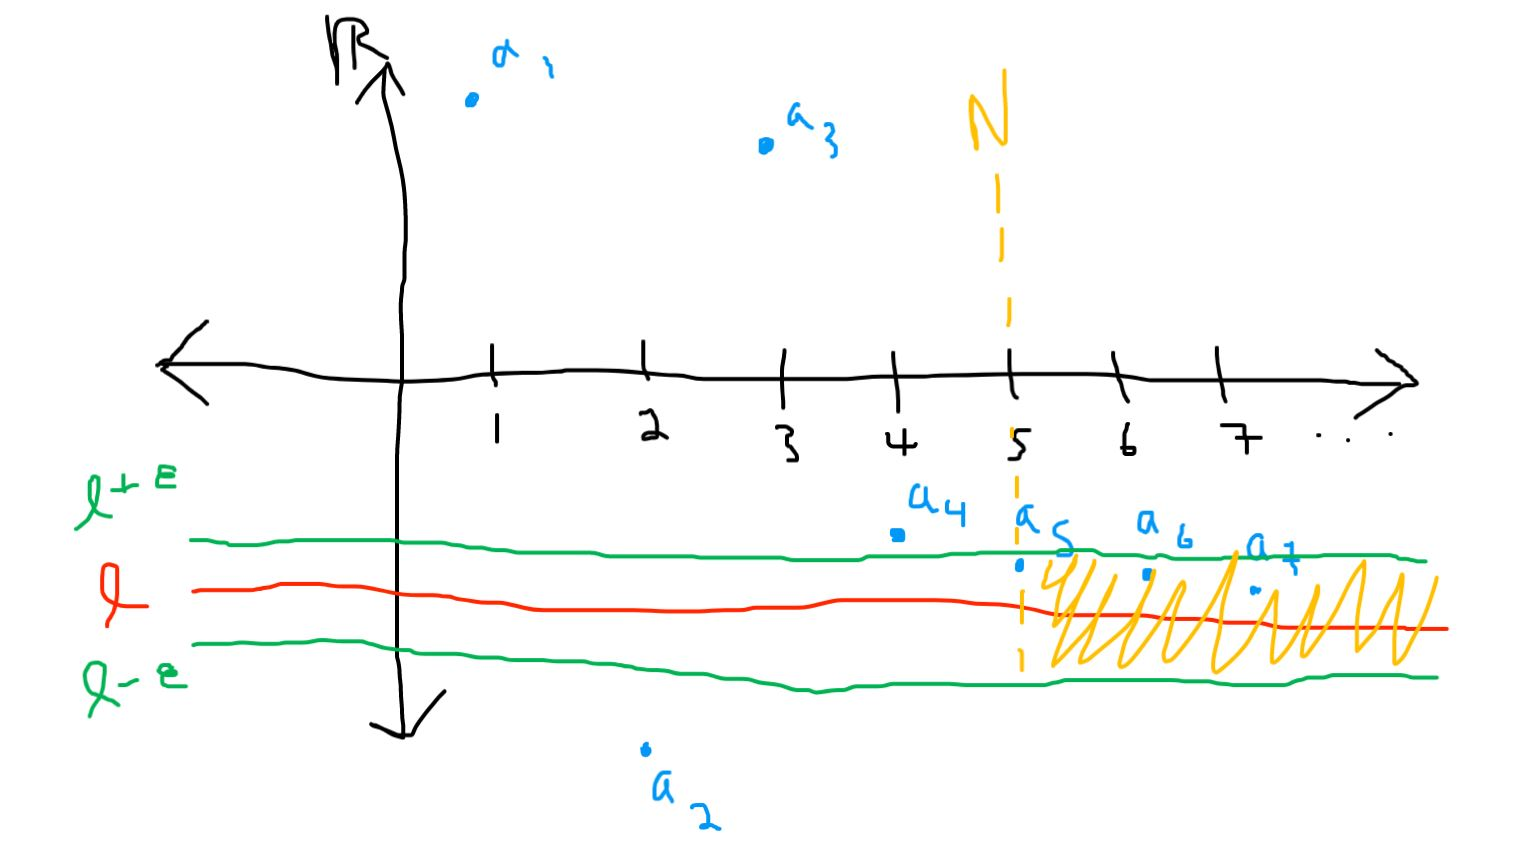
\includegraphics[width = 0.9\textwidth]{limits.JPG}
\end{center}

The idea is that the \vocab{limit} $\ell$ exists if for every $\varepsilon$ we can find some $N$ such that every element in the sequence will fit within the strip $(\ell - \varepsilon, \ell + \varepsilon)$ from $a_N$ forwards.

\begin{theorem}
    Suppose $\{a_n\}, \{b_n\}_{n = 1, 2, \ldots}$ are convergent. Then $\{a_n + b_n\}_{n = 1, 2, \ldots}$ is also convergent and $\limn(a_n + b_n) = \limn a_n + \limn b_n$.
\end{theorem}

\begin{proof}
    For brevity let $\alpha:= \limn a_n, \beta:= \limn b_n$. Consider arbitrary $\varepsilon > 0$. Then for sufficiently large $n$ we have
    \begin{align*}
        \abs{(a_n + b_n) - (\alpha + \beta)} &= \abs{(a_n - \alpha) + (b_n - \beta)} \\
        &\le \abs{a_n - \alpha} + \abs{b_n - \beta} \\
        &< \frac{\varepsilon}{2} + \frac{\varepsilon}{2} \\
        & = \varepsilon.
    \end{align*}
    We are able to do this because the definition of the limit guarantees that there exists some $M\in \NN$ such that $\abs{a_n - \alpha} < \frac{\varepsilon}{2}$ for all $n\ge M$, and similarly there exists some $N\in \NN$ such that $\abs{a_n - \alpha}$ for all $n\ge N$. Thus, we can simply pick $n\ge \max\{M, N\}$, and since $\varepsilon$ was arbitrary, we're done.
\end{proof}

\begin{theorem}
    Suppose $\{a_n\}$ is convergent. Then it is also bounded.
\end{theorem}
\begin{proof}
    The definition of the limit with $\varepsilon = 1$ guarantees that there exists $N\in \NN$ such that $\abs{a_n - \ell} < 1$ for all $n\ge N$. I claim that $L = \max \{1 + \abs{\ell}, \abs{a_1}, \ldots , \abs{a_{N - 1}}\}$ is the upper bound. There are two cases. For all $n\in \{1, 2, \ldots , N - 1\}$, we have
    \[\abs{a_n} \le \max \{\abs{a_1}, \ldots , \abs{a_{N - 1}}\}\le L.\]
    For all $n\ge N$, we have $\abs{a_n} = \abs{a_n - \ell + \ell} \le \abs{a_n - \ell} + \abs{\ell}$ by the Triangle Inequality, so $\abs{a_n} < 1 + \abs{\ell}\le L$ by the definition of $L$, so for all $n\in \NN$, $\abs{a_n}\le L$ as desired.
\end{proof}

\begin{theorem}
    Suppose $\{a_n\}, \{b_n\}$ are convergent. Then $\{a_nb_n\}$ is also convergent and furthermore $\limn(a_nb_n) = \limn a_n \limn b_n$.
\end{theorem}

\begin{proof}
    Let $\alpha = \limn a_n, \beta = \limn b_n$. Let $\varepsilon > 0$ be arbitrary. Since $\{b_n\}$ converges, it is also bounded, so there exists $L\in \RR$ such that $\abs{b_n} \le L$ for all $n\in \NN$. On the other hand, from $a_n\to \alpha$, there exists $M\in \NN$ such that $\abs{a_n - \alpha} < \frac{\varepsilon}{1 + \abs{\alpha} + \abs{L}}$ for all $n\ge M$, and similarly there exists $N\in \NN$ such that $\abs{b_n - \beta} < \frac{\varepsilon}{1 + \abs{\alpha} + \abs{L}}$. Then for all $n\ge \max \{M, N\}$, we have
    \begin{align*}
        \abs{a_nb_n - \alpha\beta} &= \abs{a_nb_n - \alpha b_n + \alpha b_n - \alpha\beta} \\
        &= \abs{(a_n - \alpha)b_n + \alpha(b_n - \beta)} \\
        &\le \abs{a_n - \alpha}\abs{b_n} + \abs{\alpha}\abs{b_n - \beta} \\
        &< \frac{\varepsilon}{1 + \abs{\alpha} + \abs{L}}\cdot \abs{L} + \abs{\alpha}\cdot \frac{\varepsilon}{1 + \abs{\alpha} + \abs{L}} \\
        &= \frac{\varepsilon(\abs{\alpha} + \abs{L})}{1 + \abs{\alpha} + \abs{L}} \\
        &< \varepsilon
    \end{align*}
    as desired.
\end{proof}
\end{document}